\section{Exploring the Design Space of Text Input in VR}

\subsection{Challenges of Text Entry in Virtual Reality}

Text entry using a physical keyboard is a complex interaction that involves the placement of the user's hands, the kinaesthetic feedback of fingers, and the physical constraints of the keyboard~\cite{McGill:2015:DRO:2702123.2702382}.
Together this interaction is able to create an efficient text entry mechanism.

However, in the context of virtual reality, it is often not possible to use a physical keyboard.
Additionally, it is desirable to be able to type with existing virtual reality specific input devices, so the user doen't have to remove the head-mounted display to type. 
In this next section we explore the challenges of text in virtual reality.

\subsubsection{Latency in Visual Feedback}
Typing is complex interaction that requires a high-bandwidth feedback loop~\cite{McGill:2015:DRO:2702123.2702382}.
Latency is a barrier in achieving a seamless interaction between the real and virtual~\cite{leedesigning}.

In virtual reality, latency is the time between movement of the and the updated image being displayed on the screen.  
This pipeline includes the times for fusion, image transmission, rendering, sensor response and display response.
This is commonly referred to as the \textit{motion-to-photon} latency.

To achieve a genuine sense of presence~\cite{schuemie2001research} in virtual reality, the total \textit{motion-to-photon} latency must be less than 20 milliseconds~\cite{jerald2009relating,jerald2010scene,bailey2004latency}.
Some existing systems have a latency as high as 80 milliseconds ~\cite{lincoln2016motion,dallaire2016animated}.

Compared to head movement, touch-based interactions need even tighter tolerances on latency.
Research on touchscreens finds that for a user to perceive display elements as naturally being affected by touch, there is a perceptual floor between 2  and 11 milliseconds below which users do not notice lag~\cite{Jota:2013:FFE:2470654.2481317,Ng:2012:DLD:2380116.2380174}.
Further, for dragging interactions, a latency of 2.38 milliseconds is required to give the perception of a natural interaction~\cite{Jota:2013:FFE:2470654.2481317,Ng:2012:DLD:2380116.2380174}.

\subsubsection{Limited Proprioception}
Manipulation in virtual reality is difficult because users must do without the haptic contact with keyboard buttons they rely on in the real world to orient themselves.
Interactions involving the body and the external world become difficult.
For example, even the simple task of placing the finger on the correct key can become difficult given the lack of proprioceptive sensations in virtual reality.

\subsubsection{Reduced Precision}
Haptic feedback and physical constraints in real world input devices help to define interactions. 
Fine-grained control is difficult in virtual reality and restricts users to the coarse manipulation of virtual objects.
Input devices that excluded the use of the fingers are slower~\cite{Zhai:1996:IMG:238386.238534}.  

\subsection{Initial Experimentation}

Our exploration of virtual reality input methods starts by building a few prototypes.
With each prototype, we ask 3 to 5 users to type a few sentences.  
For each test we give little to no instruction about how the input method works and try to let the user interact with it naturally.
The goals of this prototyping process is to explore the performance potential of each input device and to investigate if users could understand the visual interface.
We record typing speeds, their understanding of the input device, and their verbal feedback.

\subsection{Design \#1 - Gaze Input}
Many virtual reality apps today use a gaze keyboard for text entry~\cite{netflix_app_for_oculus}.
A virtual keyboard is presented in virtual reality.
The users types a letter by gazing at the desired key and tapping on a button located on the side of the head mounted display.
Users find the process slow and the motion of the head with the fixed keyboard can causes nausea and dizziness~\cite{atienza2016interaction}.
We found users type around 10 words per minute using this method.

\subsection{Design \#2 - Drumming}
Google models typing as drumming~\cite{google_drums}.
Controllers in the real world are mapped to drum sticks in the virtual world.  
Typing a character means hitting one of 26 drums laid out like a keyboard.
Users find it fun.
It could be difficult to hit the correct key and the constant arm movement some users found to be strenuous.
We found users type around 20 words per minute using this method.

\subsection{Design \#3 - External Camera}

We next explore the use of a virtual keyboard on a touchscreen, the input method used on mobile phones today.
To address the problem that we cannot see our fingers in virtual reality, we experimented with mixed reality (augmented plus virtual) with a camera.
Our prototype points the front facing camera on the head mounted display points at the mobile keyboard, and streams the view of our fingers and the keyboard into the virtual environment. 

The goal of this prototype is to investigate how latency and presence, particular of the fingers, affect performance.
We found that the latency is an inhibitor to fast input.
Our fingers are so fast that we can only see where our fingers were.
What we see is constantly wrong and just makes it even harder to type.
This prototype demonstrates how challenging the visual latency is for typing. 
We found users type around 10 words per minute using this method.


\begin{figure}[!htb]
  \centering

  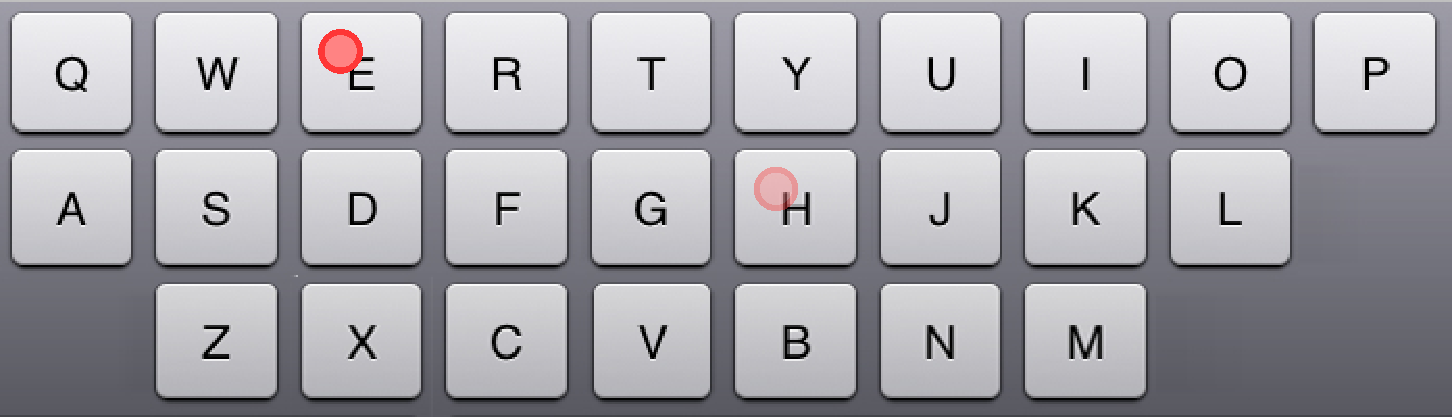
\includegraphics[width=1\columnwidth]{figures/26-Tap}

  \caption{The 26-Key tap keyboard design.}
  ~\label{fig:multiword}
\end{figure}

\subsection{Design \#4 - 26-Key Tap}

In this experiment, we explore how feedback can be added to a soft keyboard on the mobile phone to make it usable in virtual reality.
We want to explore the limit of touch typing and muscle memory for a user in a virtual enviroment.
We build a prototype keyboard, shown in Figure~\ref{fig:gesture}, for a mobile phone that transmits to the head-mounted display when where the user touches on the keyboard.
In this way, the user gets feedback where a finger is located on the keyboard with every tap.
The prototype keyboard is running alongside the standard Android keyboard that includes autocorrect to adjusted for typos and phonetic misspelling.

We notice an unexpected phenomenon using this prototype.
Even hitting the same key twice is difficult.
Every time a user lifts a finger and lowers the finger, there is a nontrivial chance that the finger has drifted to another key.
Even though the keyboard layout is familiar, and even error correction is applied, the error rate in this method make it unusable.
From this experiment, we hypothesize that for fine motor skills, some degree of either visual or haptic feedback is needed.


\begin{figure}[!htb]
  \centering

  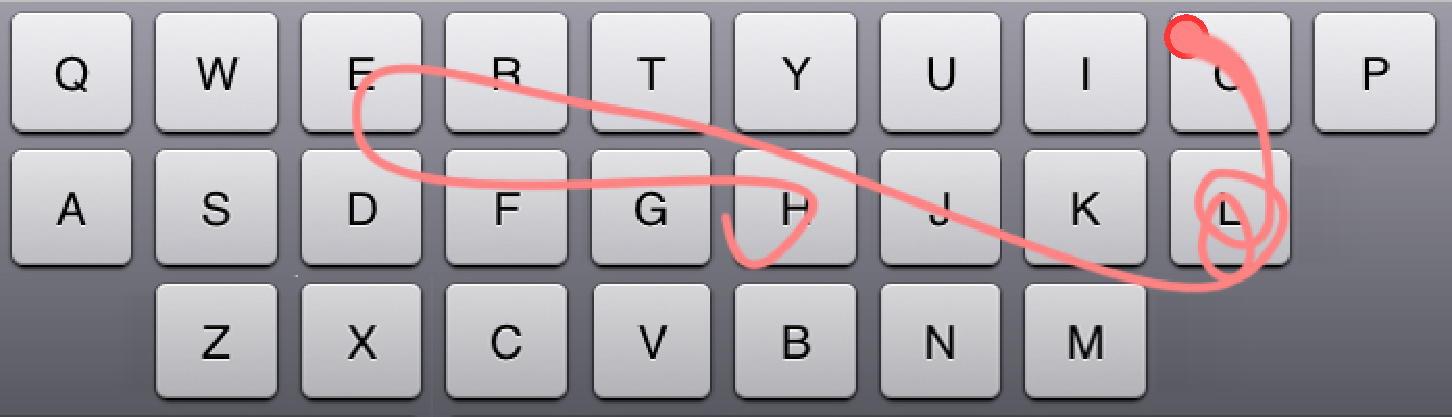
\includegraphics[width=1\columnwidth]{figures/gesture}
  
  \caption{The 26-Key gesture keyboard design.}
  ~\label{fig:gesture}
\end{figure}

\subsection{Design \#5 - 26-Key Gesture}


Gesture keyboards are shown to be effective in speeding up typing on mobile devices.
Since it does not involve lifting the finger, we postulated that it may also be useful in virtual reality.
Similar to the 26-key tap, the layout of the mobile QWERTY keyboard is preserved, except tapping is replaced by dragging to specific keys.
We show the virtual keyboard and gesture trail to indicate where the finger was in the virtual enviroment, shown in Figure~\ref{fig:gesture}.
We find that gestures works better than tapping.  However, there are two main problems: 

Firstly, the users cannot get the first letter right when starting the gesture.  We modify the shape recognition algorithm to as follows.  When the user puts their finger on the mobile screen, it always starts in the center.
The first inflection point is then discarded and the rest of the input is then done at the mobile phone system level using the standard gesture keyboard.

However, the speed with which the user creates gestures with the head-mounted display on is around three times slower than with the head-mounted display off.
Even for users that are familiar with gesture keyboards on their mobile phone, it is difficult for them to generate gestures in an efficient manner in virtual reality.
%Shape, location, and bi-gram modeling is used by SHARK2~\cite{kristensson2004shark} to generate the n-best outputs.

In summary, the use of gesture keyboard over a conventional keyboard is the best among the choices we explored in the initial phase.
Nonetheless, the speed of around 23 words per minutes is still lower than desired.


\begin{comment}
>
\subsection{Design \#4 - 8-key Drag}
\vspace*{.1cm}
\includegraphics[width=.9\columnwidth]{figures/26Tap}

QWERTY keyboard is broken into 8 regions instead of 6.
User interact with this keyboard through dragging.
Both hands are required, with each hand dragging four directions (left, up, right, down) to input the 8 regions.

\subsection{Design \#5 - 6-key Tap}
\vspace*{.1cm}
\includegraphics[width=.9\columnwidth]{figures/26Tap}

This is our first design utilizing batched keys. QWERTY keyboard is divided into 6 sections. Tapping corresponding regions triggers input for a whole section.
A word recommender algorithm in back end is required.


\subsection{Design \#6 - 6-key Drag}
\vspace*{.1cm}
\includegraphics[width=.9\columnwidth]{figures/26Tap}

Similar to 6 keys tap, the method of interaction is changed to drag instead of tap.
A word recommender algorithm in back end is required.

Even though there can be realistic representation of the keyboard and his fingers in VR, users still suffer from not being able to see some part of his own body.
The solution to such visual segmentation is not apparent, for whole body tracking in VR is not yet available.

Studies show that users possesses approximate knowledge of where their fingers are on screen thanks to proprioception \cite{boff1986handbook}.

\section{Design Goals}
Before describing the prototypes and lessons learned, we present five high-level design goals that focus on input metrics, user experience, and adaptability.
These goals are informed by related work and our experience building other systems.

\subsection{Efficient}
How closely does the new device approach exceed the speed of the best devices for text input in virtual reality?

\subsection{Learnable}
How long does the device take to learn?
Does it rely on existing skills?
Is there ways for the user to transition from being a novice to an expert?

\subsection{Practical}
Is the input method usable today?
Moreover, will it be usable in the future given the where we think virtual reality controller are heading?

\subsection{General}
Is the text input method useful across multiple types of applications?
Can the user type their username, password, and a message to a friend?

\subsection{Usable}
Desktop user sessions are longer than mobile~\cite{Kamvar:2009:CIM:1526709.1526817}.
We hypothesize that virtual reality will have a user session time closer to that of a desktop computer than a mobile phone.
Once a user has take the time to wear the head mounted display and controller, the session will
Will the user be able to use the text input method comfortably?
Can they use it for as long as they use as they their computer at night?


\end{comment}

